% Тут используется класс, установленный на сервере Papeeria. На случай, если
% текст понадобится редактировать где-то в другом месте, рядом лежит файл matmex-diploma-custom.cls
% который в момент своего создания был идентичен классу, установленному на сервере.
% Для того, чтобы им воспользоваться, замените matmex-diploma на matmex-diploma-custom
% Если вы работаете исключительно в Papeeria то мы настоятельно рекомендуем пользоваться
% классом matmex-diploma, поскольку он будет автоматически обновляться по мере внесения корректив
%
\documentclass{matmex-diploma}
\begin{document}
% Год, город, название университета и факультета предопределены,
% но можно и поменять.
% Если англоязычная титульная страница не нужна, то ее можно просто удалить.
\filltitle{ru}{
    chair              = {Кафедра системного программирования},
    title              = {Абстрактный лексический анализ},
    type               = {coursework},
    position           = {студентки},
    group              = 344,
    author             = {Вербицкой Екатерины Андреевны},
    supervisorPosition = {аспирант кафедры системного программирования},
    supervisor         = {С. В. Григорьев},
%   reviewerPosition   = {ст. преп.},
%   reviewer           = {А.А. Привалов},
%   chairHeadPosition  = {д.\,ф.-м.\,н., профессор},
%   chairHead          = {К.Х. Хунта},
%   university         = {Санкт-Петербургский Государственный Университет},
%   faculty            = {Математико-механический факультет},
%   city               = {Санкт-Петербург},
%   year               = {2013}
}
\maketitle
\tableofcontents
% У введения нет номера главы
\section*{Введение}
Многие современные языки программирования позволяют во время выполнения
формировать в виде строк выражения на других языках и выполнять их. Наиболее 
распространённые примеры — встроенный SQL (частный случай — динамический SQL~\cite{ISO}),
генерация HTML, различные DSL. Важной характеристикой таких динамически 
формируемых выражений является то, что это выражения на некотором языке 
программирования, обычно называемом встроенным языком, и с ними возникают те же
проблемы, что и при разработке на обычном языке. Одна из основных трудностей — 
отсутствие возможности статической проверки корректности динамически формируемых
выражений, и, как следствие, выявление ошибок происходит лишь во время выполнения
программы. Это существенно увеличивает затраты на разработку, отладку и 
сопровождение приложений, в которых используются встроенные языки. Кроме того, 
встроенные языки являются серьёзным источником уязвимостей информационных 
систем. Например, атаки основанные на SQL-инъекциях возможны благодаря 
использованию в приложениях встроенного SQL.

С другой стороны, при разработке приложений сейчас используются современные 
интегрированные среды разработки, которые предоставляют разработчику набор 
различной функциональности, позволяющей значительно упростить процесс разработки. 
Например автодополнение, различные рефакторинги, дополнительные статические 
проверки и подсказки. Для встроенных языков такая функциональность так же была 
бы очень полезной.

Область статической обработки встроенных языков является достаточно молодой и, 
несмотря на то, что уже существуют реализации инструментов для работы с 
динамически формируемыми выражениями  (например Java String Analyzer (JSA)~\cite{JSA}, 
Alvor~\cite{Alvor} или PHP String Analyzer~\cite{PHPSA}), есть необходимость в разработке 
различных инструментальных средств для работы со встроенными языками. Одними из 
важных шагов большинства таких инструментов является  лексический и 
синтаксический анализы для построения структурного представления динамически 
формируемых выражений для дальнейшего анализа. Промышленный подход к разработке, 
опираясь на опыт разработки инструментов для работы с обычными языками 
программирования, где для разработки анализаторов традиционно используются 
средства, упрощающие процесс, такие как генераторы лексических и синтаксических 
анализаторов, требует создания аналогичных генераторов и для встроенных языков. 
Однако, анализы встроенных языков имеют ряд особенностей и на текущий момент 
средства для автоматической генерации анализаторов отсутствуют.

Отдельным важным вопросом является выбор и оптимальная реализация алгоритмов 
лексического и синтаксического анализа для встроенных языков.

Целью данной работы является создание генератора лексических анализаторов для 
встроенных языков. Далее будет представлен алгоритм абстрактного лексического 
анализа на основе конечного преобразователя~\cite{FST} (Finite State Transducer или 
FST) и основанный на нём генератор абстрактных лексических анализаторов. 
Так же представлены результаты апробации на примере создания анализатора для 
языка T-SQL. 



\section{Постановка задачи}
Целью данной работы является создание генератора абстрактных лексических 
анализаторов и его дальнейшая апробация на примере языка T-SQL. В рамках работы 
поставлены следующие задачи: 
\begin{itemize}
    \item Продумать архитектуру генератора и определить структуру входных и 
    выходных данных.
    \item Разделить процесс создания управляющих конструкций для интерпретатора
    и процесс лексического анализа.
    \item Изучить различные FST и выбрать наиболее подходящий для решаемой 
    задачи.
    \item Реализовать генератор абстрактных лексических анализаторов.
    \item Провести апробацию реализованного решения.
\end{itemize}


\section{Обзор}
\subsection{Алгоритмы абстрактного лексического анализа}

В результате работы лексического анализатора хочется иметь граф токенов, 
соответствующих спецификации обрабатываемого языка, каждый путь по которому есть 
результат лексического анализа какого-либо выражения на встроенном языке из 
начального множества.

Существует несколько подходов, используемых для осуществления лексического 
анализа динамически формируемых выражений, среди которых был выбран анализ при 
помощи конечного преобразователя. Конечный преобразователь (finite-state 
transducer) — это конечный автомат, который может выводить конечное число 
символов для каждого входного символа~\cite{ТФЯИТ}. В зависимости от типа 
отображения во множество слов выходного алфавита конечные преобразователи 
делятся на 2 типа: преобразовывающие входной поток к строковому выражению 
(string-to-string) или вычисляющие некоторую весовую функцию (string-to-weight)~\cite{FST}. 
Так как результатом работы лексического анализатора должен являться граф, 
имеющий на ребрах токены, мы будем использовать конечный преобразователь первого 
типа. 

Формально конечный преобразователь типа string-to-string есть семерка 
(Q, i, F, $\Sigma$, $\Delta$, $\sigma$, $\delta$), где: Q — множество состояний,
i $\in$ Q — начальное состояние, F $\subset$ Q — множество конечных состояний, 
$\Sigma$ — входной алфавит, $\Delta$ — выходной алфавит, $\delta$ — отображение 
типа Q $\times$ $\Sigma$ $\rightarrow$ Q, $\sigma$ — отображение типа Q $\times$ 
$\Sigma$ $\rightarrow$ $\Delta$*. 
Среди string-to-string FST выделяют секвенциальные (каждому состоянию и каждому 
символу входного алфавита соответствует единственный образ при отображениях 
$\delta$ и $\sigma$), p-сабсеквенциальные (для конечных состояний может существовать 
несколько альтернативно генерируемых строк выходного потока), а так же 
недетерминированные конечные преобразователи, которые не могут быть представлены 
в виде комбинации p-сабсеквенциальных. 

Для проведения абстрактного лексического анализа желательно иметь множество 
динамически формируемых в результате работы приложения выражений. Так выражения 
могут являться строковыми литералами, могут получаться из них посредством 
безусловной или условной конкатенации, добавления фрагментов строки в циклах или 
в рекурсии; при этом в общем случае задача точного вычисления такого множества 
неразрешима, поэтому мы будем пользоваться некоторым его конечным представлением 
в виде направленного ациклического графа.

\subsection{Генераторы лексических анализаторов}
При разработке инструментов для анализа языков программирования обычно 
используются генераторы лексических анализаторов, которые по спецификации лексики 
на специальном языке генерируют лексический анализатор обрабатываемого языка. 
При этом обычно в одном файле генерируется как управляющая информация: описание 
автомата, пользовательский код, так и интерпретатор (сам автомат).  Это 
происходит по двум причинам. Во-первых, такой подход упрощает отладку целевого 
анализатора, во-вторых большинство современных инструментов создавались для языков, 
не поддерживающих функциональную парадигму, что создавало проблемы при попытке 
разделить генерацию пользовательского action-кода и статическую реализацию ядра 
алгоритма анализа.

Инструментов, генерирующих лексические анализаторы для встроенных языков на 
данный момент не существует. В рамках работы~\cite{МГСВ} было показано, что для 
лексического анализа динамического SQL можно переиспользовать уже существующую 
спецификацию лексера для основного языка без модификаций (основной язык тоже 
SQL). В рамках этой работы была предпринята попытка использовать стандартный 
лексер, сгенерированный FsLex-ом по уже существующей спецификации. Лексеру на 
вход подавали строку на ребре входного графа и на выходе получали последовательность 
токенов, которую преобразовывали в путь в графе. Однако, при таком подходе 
возникают сложности с “рваными” литералами, т.е. такими ситуациями, когда 
различные части одной лексической единицы содержатся на различных рёбрах графа. 
Например, в одном из проектов, в рамках которого решалась задача миграции 
хранимого кода с MS-SQL Server на Oracle, количество динамических запросов 
составляло более 3000 и из них 120 не проходили лексический анализ по причине 
наличия “рваных” литералов~\cite{МГСВ}. Предлагаемое в работе 
решение  данной проблемы, основанное на склейке цепочек рёбер в одно, является 
очень ресурсоёмким на реальных графах и не позволило полностью решить проблему.

В работе~\cite{ToDetect} показано, что можно использовать FST, построенный стандартным 
генератором, однако полноценного генератора не реализовано.

Таким образом, возможно попытаться создать генератор абстрактных лексических 
анализаторов на основе существующих генераторов. В рамках данной работы в 
качестве основы был выбран JFlex — популярный генератор лексических анализаторов 
для языка Java. Выбор обусловлен тем, что инструмент разрабатывался под платформу 
JVM и JFlex на текущий момент является самым популярным генератором с открытым 
исходным кодом для этой платформы. Доступность исходного кода важна, так как 
необходима модификация самого генератора.

\section{Реализация}
\subsection{Терминология}
В нашем случае структурой данных, с которую подучает на вход абстрактный 
синтаксический анализатор, будет граф, являющийся представлением результата 
протягивания констант. Таким образом каждому пути в графе соответствует некоторое 
возможное значение динамического запроса. Будем говорить, что данный путь 
порождает соответствующее значение.

Будем говорить, что запрос содержит лексические или синтаксические ошибки, 
если в графе, соответствующем этому запросу, существует хотя бы один путь, 
порождающий значение с лексической или синтаксической ошибкой соответственно.

В рамках решаемой задачи основной структурой данных для лексического и 
синтаксического анализа является граф. Его можно воспринимать как аналог 
входного потока символов для лексического анализатора и потока токенов для 
синтаксического. Поэтому мы будем говорить о токенизации или лексическом анализе 
графа, подразумевая под этим некоторый процесс, который переведёт граф, 
содержащий строки, в граф, содержащий токены. Аналогичным образом мы будем 
говорить о синтаксическом анализе (разборе) графа, подразумевая процесс, на 
выходе которого мы получаем некоторое множество синтаксических деревьев или лес, 
соответствующих входному графу. Каждое дерево соответствует некоторому значению 
запроса, порождённому некоторым путём во входном графе. Таким образом дерево 
соответствует пути в графе.

\subsection{Генерация абстрактных лексических анализаторов}
В рамках проекта лаборатории JetBrains, целью которого является создание 
платформы для анализа кода на встроенных языках, был реализован генератор 
лексических анализаторов, который, в отличие от классических инструментов типа 
Lex, порождает лексический анализатор, принимающий на вход граф, который 
является компактным представлением множества значений динамически формируемого 
выражения. Результатом работы такого анализатора является граф, собранный из 
токенов, встречающихся в строках, содержащих встроенный код. В качестве 
основного языка реализации был выбран язык программирования Scala~\cite{Scala}, так как 
поддержка функциональной парадигмы заметно упрощает решение задач, связанных с 
различными анализами кода, в том числе и лексическим.

В качестве основы для генератора был использован генератор лексических 
анализаторов для Java — JFlex~\cite{JFlex}. Для него реализована генерация управляющих 
данных (описание конечного автомата, пользовательский код) в язык 
программирования Scala, для чего пришлось модифицировать JFlex. При этом была 
отделена функция токенизации, которая в нашей реализации не генерируется, а 
реализована статически и параметризуется сгенерированными данными. Таким образом, 
полный цикл работы с инструментом выглядит следующим образом:
\begin{figure}[h]
 \label{Arch}
 \centering
 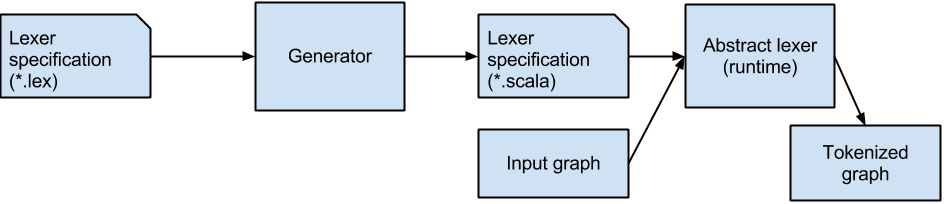
\includegraphics[width=15cm]{AL_base_arch.png}
 \caption{Архитектура решения}
 \label{Arch}
\end{figure}

\subsection{Интерпретация управляющих конструкций}
Для проведения абстрактного лексического анализа желательно иметь множество 
динамически формируемых в результате работы приложения выражений. Так выражения 
могут являться строковыми литералами, могут получаться из них посредством 
безусловной или условной конкатенации, добавления фрагментов строки в циклах 
или в рекурсии; при этом в общем случае задача точного вычисления такого множества 
неразрешима, поэтому мы будем пользоваться некоторым его конечным представлением 
в виде направленного ациклического графа.

Входной структурой данных для лексического анализатора является граф, являющийся 
представлением множества возможных значений конкретного динамически формируемого 
выражения. На рёбрах этого графа хранятся строки, соответствующие значениям 
переменных из которых формировалось выражение. Результатом работы анализатора 
является граф, пригодный для дальнейшего синтаксического анализа, каждое ребро 
которого может либо содержать токен, либо эпсилон-ребром.

Ниже изложен ряд принятых нами ограничений на входные данные, которые далее 
считаются верными, если не оговорено иное.
\begin{itemize}
    \item Обрабатываемый граф является DAG-ом. Данное упрощение сделано на 
    основе практического наблюдения, что при раскрытии цикла в единственное 
    повторение не нарушается синтаксическая корректность и учитываются все 
    переменные, участвующие в построении запроса. Этого достаточно для того, 
    чтобы решить задачу трансляции. 
    \item У DAG-а одна стартовая и одна конечная вершина. Для конечной вершины 
    верно, что из неё не выходит ни одна дуга. Это достигается явным добавлением 
    дуги с токеном, обозначающим конец ввода (EOF).
\end{itemize}

Абстрактный лексер основан на конечном преобразователе (finite state transducer, 
FST~\cite{FST}), который, основываясь на сгенерированном описании автомата, переводит 
входной граф, в граф, содержащий соответствующие спецификации токены. 

Шаги лексического анализа выглядит следующим образом.
\begin{itemize}
    \item На вход подаётся граф, составленный на основе дерева разбора исходного 
    кода программы: на ребрах — фрагменты строк кода на встроенном языке, 
    вершинам соответствуют случаи конкатенации строк.
    \item Входной граф преобразовывается к виду, удобному для лексического 
    анализа: каждое ребро входного графа разбивается на последовательность новых 
    ребер, метки которых содержат только по одному символу из строки исходного 
    ребра.
    \item Запускается процедура токенизации на преобразованном графе, в 
    результате чего получается новый граф, на ребрах которого находятся 
    накопленные в результате работы абстрактного лексического анализатора 
    токены, соответствующие грамматике анализируемого встроенного языка.
\end{itemize}

Рассмотрим следующий пример исходного кода:

\begin{verbatim}
IF @X = @Y
    SET @TABLE = '#tbl1'
ELSE
    SET @TABLE = 'tbl2'
    SET @S = 'SELECT x FROM' + @TABLE
EXECUTE (@S)
\end{verbatim}

По нему будет построен граф, представленный на рисунке~\ref{SimpleSql}:
\begin{figure}[h]
 \label{SimpleSql}
 \centering
 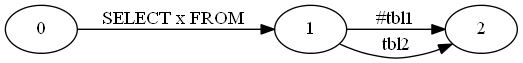
\includegraphics[width=15cm]{SimpleSql.dot.png}
 \caption{Входной граф}
 \label{SimpleSql}
\end{figure}

Граф, полученный в результате применения к нему процедуры токенизации будет 
показан на рисунке~\ref{SimpleSqlLex}.
\begin{figure}[h]
 \label{SimpleSqlLex}
 \centering
 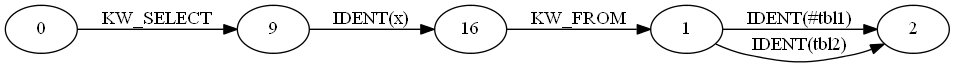
\includegraphics[width=15cm]{SimpleSql_lex.dot.png}
 \caption{Граф, полученный в результате работы абстрактного лексического анализатора}
 \label{SimpleSqlLex}
\end{figure}

\subsection{Апробация}
Реализованное решение было протестировано на примере создания лексического 
анализатора для встроенного T-SQL. В рамках апробации были выполнены следующие 
шаги. 
\begin{itemize}
    \item Задана спецификация лексики языка T-SQL на языке JFlex, которая в 
    качестве action-кода содержит конструирование токенов, описанных в 
    синтаксическом анализаторе, полученном по реальной грамматике T-SQL.
    \item По заданной спецификации сгенерирован набор управляющих конструкций 
    для анализатора на языке Scala.
    \item Создан тестовый проект, являющийся примером.
    \item Проведён ряд тестов, подтверждающих корректность полученного 
    анализатора. Для проведения тестов был подготовлен ряд входных графов, 
    представляющих основные интересные случаи.
\end{itemize}

Наиболее важным тестом являлась проверка обработки рваных литералов. Для 
демонстрации ниже приведены входной и выходной графы, содержащие рваные 
литералы и результат их обработки.
\begin{figure}[h]
 \label{Literals}
 \centering
 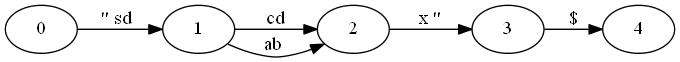
\includegraphics[width=15cm]{Literals_1.dot.jpg}
 \caption{Входной граф, содержащий рваные литералы}
 \label{Literals}
\end{figure}

\begin{figure}[h]
 \label{LiteralsLex}
 \centering
 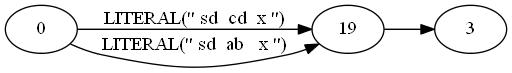
\includegraphics[width=15cm]{Literals_1_lex.dot.jpg}
 \caption{Результат работы абстрактного лексического анализатора для графа, 
    представленного на рисунке~\ref{Literals}}
 \label{LiteralsLex}
\end{figure}

Таким образом, в ходе экспериментов было показано, что реализованный инструмент 
позволяет по спецификации сгенернировать абстрактный лексический анализатор 
заданного языка, корректно обрабатывающий ситуации с рваными литералами.


% У заключения нет номера главы
\section*{Заключение}
В ходе выполнения данной работы были получены следующие результаты: 
\begin{itemize}
    \item Изучены различные FST, выбран подходящий для решаемой задачи.
    \item Продумана архитектура генератора абстрактных лексических анализаторов:
    \begin{itemize}
        \item определена структура входных и выходных данных;
        \item разделен процесс создания управляющих конструкций для 
        интерпретатора и процесс лексического анализа.
    \end{itemize}
    \item Реализован генератор абстрактных лексических анализаторов.
    \item Проведена апробация реализованного решения.
    \item Результаты работы были успешно представлены на конференции 
    “СПИСОК-2013”. Тезисы опубликованы в сборнике материалов конференции.
\end {itemize}

Исходный текст результатов моей работы можно получить по адресу 

https://code.google.com/p/string-embedded-languages-analysis-platform/

Имя пользователя, под котоорым работал автор: kajigor.

\subsection*{Дальнейшее направление работы}
На практике далеко не каждый случай использования встроенных языков может быть 
представлен в виде направленного ациклического графа.  В дальнейшем будет
исследован вопрос необходимости поддержки произвольных входных графов. Если
она окажется необходимым, то будут  внесены соответствующие изменеия в алгоритм
анализа. Так же планируется реализация 
механизма сообщения об ошибках. Следующим этапом после проведения лексического 
анализа является синтаксический анализ, для которого в свою очередь потребуется 
генератор абстрактных синтаксических анализаторов, работу над реализацией 
которого планируется провести далее в рамках проекта. 


\bibliographystyle{ugost2008ls}
\bibliography{course_work.bib}
\end{document}